\documentclass[10pt,a4paper]{article}

% ================================================================ fonts
\usepackage[T1]{fontenc}
\usepackage[utf8]{inputenc}
\usepackage[default,semibold]{sourceserifpro}   % body
\usepackage[scale=0.95]{inter}                  % headings, captions, UI
\usepackage[scale=0.84]{sourcecodepro}          % code
\usepackage[varbb]{newtxmath}
\newcommand{\hfont}{\sffamily}

% ================================================================ layout
\usepackage[a4paper,top=24mm,bottom=26mm,inner=24mm,outer=24mm,
            headsep=8mm,footskip=12mm]{geometry}
\usepackage{microtype}
\linespread{1.08}
\setlength{\emergencystretch}{2.5em}
\setlength{\parindent}{0pt}
\setlength{\parskip}{0.55em plus 0.1em}

% ================================================================ packages
\usepackage{amsmath}
\usepackage{booktabs}
\usepackage{tabularx}
\usepackage{multirow}
\usepackage{enumitem}
\usepackage[table]{xcolor}
\usepackage{tikz}
\usetikzlibrary{arrows.meta,positioning,calc,fit,backgrounds,shapes.misc}
\usepackage[ruled,vlined,linesnumbered]{algorithm2e}
\usepackage{listings}
\usepackage{caption}
\usepackage{titlesec}
\usepackage{fancyhdr}
\usepackage[most]{tcolorbox}
\usepackage[numbers,sort&compress]{natbib}
\usepackage[colorlinks=true,linkcolor=accent,citecolor=accent,urlcolor=accent]{hyperref}
\usepackage[capitalise,noabbrev]{cleveref}

% ================================================================ palette
\definecolor{ink}{HTML}{18181B}
\definecolor{muted}{HTML}{71717A}
\definecolor{hairline}{HTML}{E4E4E7}
\definecolor{accent}{HTML}{3F3F46}
\definecolor{accentsoft}{HTML}{F4F4F5}
\definecolor{accent2}{HTML}{71717A}
\definecolor{accent2soft}{HTML}{F4F4F5}
\definecolor{warn}{HTML}{18181B}
\definecolor{warnsoft}{HTML}{F4F4F5}
\definecolor{llmfill}{HTML}{FFFFFF}
\definecolor{llmdraw}{HTML}{27272A}
\definecolor{detfill}{HTML}{F4F4F5}
\definecolor{detdraw}{HTML}{A1A1AA}
\definecolor{loopcol}{HTML}{18181B}
\definecolor{codebg}{HTML}{F7F7F7}
\definecolor{tablehead}{HTML}{F1F1F2}
\color{ink}

% ================================================================ headings
\titleformat{\section}
  {\hfont\Large\bfseries\color{ink}}
  {\makebox[2.1em][l]{\color{accent}\secnum}}
  {0pt}{}
  [\vspace{-0.55em}{\color{hairline}\rule{\linewidth}{0.6pt}}]
\titleformat{\subsection}
  {\hfont\large\bfseries\color{ink}}
  {{\color{accent}\thesubsection}}{0.7em}{}
\titlespacing*{\section}{0pt}{1.9em}{0.9em}
\titlespacing*{\subsection}{0pt}{1.3em}{0.4em}
\makeatletter
\renewcommand{\paragraph}[1]{%
  \par\vspace{0.35em}{\hfont\bfseries\color{accent}#1}\hspace{0.6em}\ignorespaces}
\makeatother

% ================================================================ header / footer
\pagestyle{fancy}
\fancyhf{}
\renewcommand{\headrulewidth}{0pt}
\renewcommand{\sectionmark}[1]{\markboth{#1}{}}
\fancyhead[L]{\hfont\scriptsize\color{muted}\textbf{\color{accent}litresearch}\quad Iterative literature research agent}
\fancyhead[R]{\hfont\scriptsize\color{muted}\leftmark}
\fancyfoot[C]{\hfont\footnotesize\color{muted}\thepage}
\fancypagestyle{plain}{\fancyhf{}\fancyfoot[C]{\hfont\footnotesize\color{muted}\thepage}}

% ================================================================ captions, lists
\captionsetup{font={small,sf},labelfont={bf,color=accent},labelsep=quad,
              justification=raggedright,singlelinecheck=false}
\captionsetup[table]{position=top,skip=6pt}
\setlist{itemsep=3pt,topsep=4pt,parsep=0pt}
\setlist[itemize]{label={\color{accent}\textbullet}}
\setlist[description]{font=\hfont\bfseries\color{accent}}
\setlist[enumerate]{label={\hfont\bfseries\color{accent}\arabic*}}

\newcommand{\secnum}{\ifnum\value{section}<10 0\fi\arabic{section}}
\newcommand{\code}[1]{\texttt{#1}}
\newcommand{\sys}{{\hfont\bfseries litresearch}}

% ================================================================ tables
\setlength{\aboverulesep}{0pt}
\setlength{\belowrulesep}{0pt}
\renewcommand{\arraystretch}{1.3}
\newcommand{\headrow}{\rowcolor{tablehead}}
\newcommand{\tcol}[1]{{\hfont\bfseries\footnotesize\color{accent}#1}}

% ================================================================ boxes
\tcbset{
  basebox/.style={enhanced, breakable, boxrule=0pt, arc=3pt, outer arc=3pt,
    left=12pt, right=12pt, top=8pt, bottom=8pt},
}
\newtcolorbox{callout}[3][]{basebox,
  colback=#2soft, borderline west={3pt}{0pt}{#2},
  fonttitle=\hfont\bfseries\small, coltitle=#2, colbacktitle=#2soft,
  attach title to upper, title={#3\hspace{0.6em}}, after title={\par\smallskip}, #1}
\newtcolorbox{abstractbox}{basebox, colback=accentsoft,
  borderline west={3pt}{0pt}{accent}, left=16pt, right=16pt, top=12pt, bottom=12pt}

\lstset{
  basicstyle=\ttfamily\footnotesize, backgroundcolor=\color{codebg},
  frame=single, rulecolor=\color{hairline}, framesep=7pt,
  columns=fullflexible, keepspaces=true, breaklines=true,
  xleftmargin=7pt, xrightmargin=7pt, aboveskip=10pt, belowskip=4pt,
}

\SetKwComment{Comment}{$\triangleright$\ }{}
\SetAlFnt{\small}
\SetAlCapFnt{\hfont\small\bfseries}
\SetAlCapNameFnt{\hfont\small}


\begin{document}

% ================================================================ title block
\thispagestyle{plain}
\begin{tikzpicture}[remember picture,overlay]
  \fill[ink] (current page.north west) rectangle ([yshift=-6mm]current page.north east);
\end{tikzpicture}%
\vspace*{-4mm}
{\hfont\footnotesize\bfseries\color{accent}TECHNICAL REPORT\hspace{0.8em}{\color{hairline}|}\hspace{0.8em}{\color{muted}OCTOBER 2026}}

\vspace{1.0em}
{\hfont\fontsize{30}{34}\selectfont\bfseries\color{ink}litresearch}

\vspace{0.45em}
{\hfont\Large\color{muted}An iterative, state-centric agent for\\autonomous literature research}

\vspace{1.3em}
{\hfont\small\bfseries Gihan Uthpala}\hspace{0.8em}{\hfont\small\color{muted}\texttt{gihanuthpala@gmail.com}}

\vspace{0.6em}
{\color{hairline}\rule{\linewidth}{0.6pt}}
\vspace{0.4em}

% ================================================================ abstract
\begin{abstractbox}
{\hfont\footnotesize\bfseries\color{accent}ABSTRACT}\par\smallskip
Most retrieval-augmented systems treat literature search as a single
retrieval step followed by summarization. Real literature research works
differently: the investigator's understanding of the question changes as
they read, new subquestions appear, and evidence is weighed, not just
collected. We present \sys{}, an open-source agent that runs literature
research as an \emph{iterative evidence-acquisition process} over an
explicit, mutable research state. A research question is broken into a tree
of subquestions, each served by \emph{search intents} that are translated
into source-specific queries over arXiv, OpenAlex, Crossref, PubMed,
Semantic Scholar and the web. Results are merged into a canonical,
provenance-preserving document registry through a conservative four-tier
deduplication hierarchy. The registry is expanded by citation snowballing
until a saturation criterion is met, and then screened, ranked and
allocated to subquestions round-robin. Documents are read in parallel into
a structured \emph{evidence store} of claims with support, location, type
and strength. A critic reviews the state along eight dimensions and returns
\emph{research actions} rather than a binary verdict: it can add, split,
rephrase, deprioritize or close subquestions, so the research plan is an
output of the investigation as well as an input. The final report is
written section by section from the evidence store, and every citation
resolves to a retrieved document. We describe the design, the deterministic
machinery that keeps a language-model pipeline auditable, and a case study
that read 28 of 237 retrieved documents in about three and a half minutes.
We also report weaknesses the case study exposed.
\end{abstractbox}

\vspace{0.3em}
{\hfont\footnotesize\color{muted}\textbf{\color{ink}Keywords}\hspace{0.8em}
LLM agents \textperiodcentered{} literature review automation \textperiodcentered{}
retrieval-augmented generation \textperiodcentered{} citation snowballing \textperiodcentered{}
evidence synthesis \textperiodcentered{} LangGraph}
\vspace{0.6em}

% ================================================================ intro
\section{Introduction}

Large language models (LLMs) combined with retrieval have become a standard
way to answer knowledge-intensive questions~\citep{lewis2020rag}. For
\emph{literature research}, meaning the task of establishing what a body of
scholarly work says about a question, a single round of
retrieve-then-summarize falls short in three ways.

First, the right decomposition of a research question is rarely clear at
the start. It becomes clear while reading: a paper introduces terminology
the investigator did not know, shows that a subquestion has two parts that
need separate evidence, or shows that another subquestion is a dead end.
Second, the output of reading should be \emph{evidence}, not summaries. A
summary turns a paper into a single opinion. Evidence keeps each claim
separate from what supports it, so a later stage can ask whether a claim is
established by several independent studies or asserted by one. Third,
systematic reviewers have long known that keyword search alone misses
relevant work, and that following citations backward and forward is needed
for coverage~\citep{wohlin2014snowballing,kitchenham2004procedures}.

\sys{} is built around these observations. Its central design principle is
that \textbf{the research plan is not fixed}: subquestions, intents,
documents, evidence, contradictions and coverage estimates all live in one
explicit state, and every stage of the pipeline reads and changes that
state. The contributions of this paper are:

\begin{callout}{accent}{Contributions}
\begin{enumerate}[leftmargin=*]
  \item A \textbf{state-centric architecture} for literature research, in
    which a five-level hierarchy (question $\to$ subquestion $\to$ intent
    $\to$ query $\to$ source) is first-class, mutable data. Its reducers
    remain correct under parallel fan-out (\cref{sec:state}).
  \item A \textbf{conservative canonicalization hierarchy} for scholarly
    records gathered from heterogeneous sources. It uses numeral vetoes,
    Unicode folding and verified identifier lookups, so false merges, which
    silently destroy evidence, are rare (\cref{sec:canon}).
  \item \textbf{Deterministic ranking, allocation and saturation rules} that
    limit LLM calls to the points where judgement is needed. These include a
    round-robin reading allocator that prevents one subquestion from using
    up the reading budget, and a direction-aware snowballing policy
    (\cref{sec:rank,sec:snowball}).
  \item A \textbf{structured evidence store} and a \textbf{critic that
    returns plan edits}, which together close an adaptive research loop
    whose termination is controlled by both quality and budget
    (\cref{sec:evidence,sec:critic}).
  \item An \textbf{end-to-end case study} that reports what the system did,
    including several failure modes found in the process
    (\cref{sec:case}).
\end{enumerate}
\end{callout}

% ================================================================ related
\section{Background and Related Work}
\label{sec:related}

\paragraph{Retrieval-augmented and agentic LLMs.}
Retrieval augmentation conditions generation on retrieved
passages~\citep{lewis2020rag}. Agentic variants interleave reasoning with
tool use~\citep{yao2023react} or with retrieval at each reasoning
step~\citep{trivedi2023ircot,wei2022cot}. Self-reflection methods have the
model critique and revise its own output~\citep{shinn2023reflexion,madaan2023selfrefine}.
\sys{} uses reflection at the level of the \emph{research plan} rather than
the generated text: the critic's output is a set of typed edits to the
subquestion tree and new search intents, and these are applied to the state.

\paragraph{LLM systems for scholarly synthesis.}
PaperQA~\citep{lala2023paperqa} answers scientific questions by retrieving
and reading full-text papers. OpenScholar~\citep{asai2024openscholar} builds
a retrieval datastore over open-access literature for citation-backed
synthesis. STORM~\citep{shao2024storm} uses perspective-guided question
asking to outline long-form articles. Work on citation-grounded
generation~\citep{gao2023alce} shows that LLMs often cite sources that do
not support the claim. \sys{} addresses this structurally. Citations are
document identifiers taken from the evidence passed to each report section,
unresolvable identifiers are removed, and the reference list is built from
the document registry rather than generated by the model.

\paragraph{Systematic review methodology.}
Kitchenham's procedures~\citep{kitchenham2004procedures} and the PRISMA
statement~\citep{page2021prisma} formalize search, screening, eligibility
and synthesis for human-conducted reviews. Wohlin~\citep{wohlin2014snowballing}
describes backward and forward snowballing as an iterative procedure that
runs until no new relevant papers are found. \sys{} implements an
automated, budgeted version of this cycle. Its saturation criterion directly
operationalizes ``no new papers.''

\paragraph{Record linkage.}
Deduplicating bibliographic records is an instance of record
linkage~\citep{fellegi1969record,elmagarmid2007duplicate}. Our hierarchy
puts persistent identifiers first and fuzzy matching last, and it is tuned
for precision over recall. The reason is specific to this setting: a missed
duplicate costs one redundant read, while a false merge silently attributes
one paper's evidence to another.

% ================================================================ principles
\section{Design Principles}
\label{sec:principles}

Five principles shaped the implementation.

\begin{description}[leftmargin=1.2em,style=nextline]
  \item[P1. Research is a state, not a pipeline.] The state model, rather
    than the graph topology, encodes the method. Every node is a function
    from state to a \emph{delta} on state.
  \item[P2. The plan is mutable.] Subquestions carry status, priority,
    coverage and origin (\code{planner}, \code{critic} or
    \code{discovery}), and the critic can rewrite them.
  \item[P3. Evidence, not summaries.] The unit of output from reading is a
    claim paired with its support, location, type and strength.
  \item[P4. Use LLMs only for judgement.] Ranking, reading allocation,
    snowball seed selection, saturation, deduplication, termination and
    reference assembly are deterministic code, so they are testable and
    auditable.
  \item[P5. Budgets are limits, not targets.] The number of documents
    retrieved is never a stopping criterion. Budgets cap cost, and the
    critic decides sufficiency.
\end{description}

% ================================================================ architecture
\section{Architecture}
\label{sec:arch}

\sys{} is implemented as a LangGraph~\citep{langgraph} state graph
(\cref{fig:graph}). It contains two loops with different jobs. The
\textbf{inner loop} (snowball $\circlearrowleft$ screening) expands the
citation neighbourhood of documents already found and stops on a saturation
criterion. The \textbf{outer loop} (critique $\circlearrowleft$ intents) is
the adaptive research loop, and it can rewrite the research plan.

\begin{figure}[t]
\centering
\resizebox{\textwidth}{!}{%
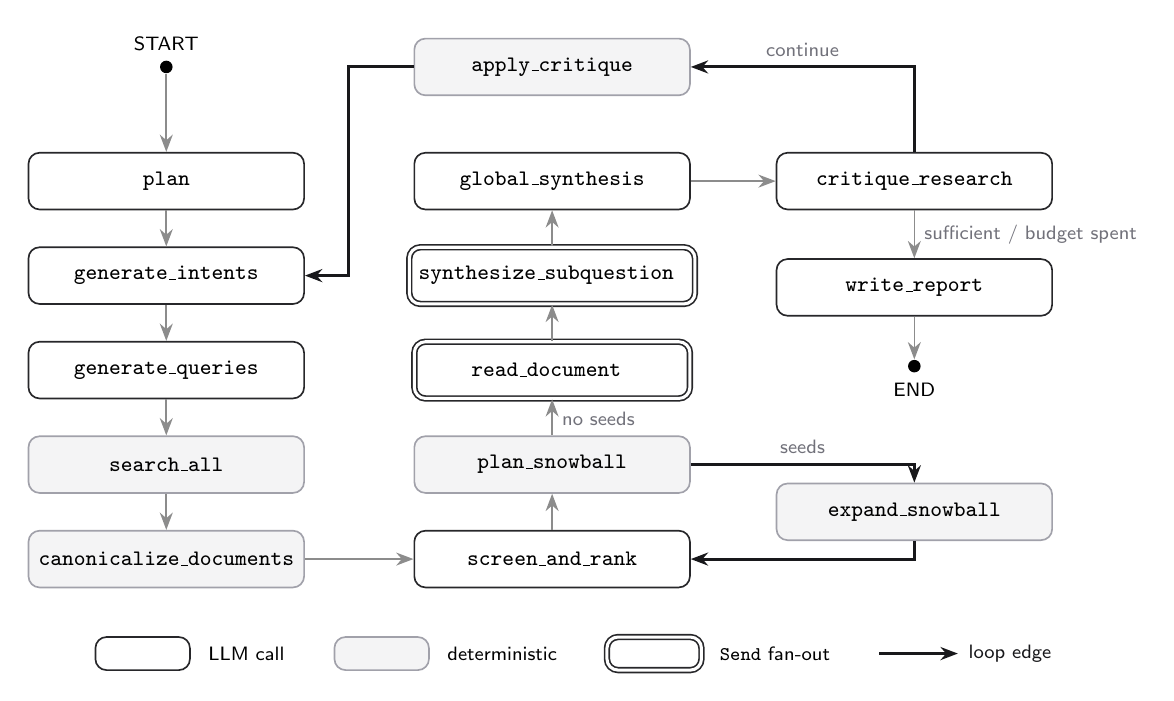
\begin{tikzpicture}[
    font=\small\sffamily,
    >={Stealth[length=2.2mm]},
    box/.style={rounded corners=4pt, minimum width=3.5cm, minimum height=0.72cm,
                align=center, line width=0.6pt, font=\ttfamily\footnotesize},
    llm/.style={box, fill=llmfill, draw=llmdraw},
    det/.style={box, fill=detfill, draw=detdraw},
    fan/.style={double, double distance=1.1pt},
    term/.style={circle, fill=black, inner sep=1.6pt},
    lbl/.style={font=\scriptsize\sffamily, text=muted},
    flow/.style={->, line width=0.6pt, draw=black!45},
    loop/.style={->, line width=1.1pt, draw=loopcol},
  ]
  % column 1: planning and retrieval
  \node[term, label={[font=\scriptsize\sffamily]above:START}] (start) at (0,1.45) {};
  \node[llm] (plan)    at (0, 0.00) {plan};
  \node[llm] (intents) at (0,-1.20) {generate\_intents};
  \node[llm] (queries) at (0,-2.40) {generate\_queries};
  \node[det] (search)  at (0,-3.60) {search\_all};
  \node[det] (canon)   at (0,-4.80) {canonicalize\_documents};

  % column 2: screening, reading, synthesis
  \node[llm] (screen)  at (4.9,-4.80) {screen\_and\_rank};
  \node[det] (snowp)   at (4.9,-3.60) {plan\_snowball};
  \node[llm,fan] (read)  at (4.9,-2.40) {read\_document $\rightrightarrows$};
  \node[llm,fan] (sqsyn) at (4.9,-1.20) {synthesize\_subquestion $\rightrightarrows$};
  \node[llm] (gsyn)    at (4.9, 0.00) {global\_synthesis};

  % column 3: snowball expansion, reflection, report
  \node[det] (expand)  at (9.5,-4.20) {expand\_snowball};
  \node[llm] (critic)  at (9.5, 0.00) {critique\_research};
  \node[det] (apply)   at (4.9, 1.45) {apply\_critique};
  \node[llm] (report)  at (9.5,-1.35) {write\_report};
  \node[term, label={[font=\scriptsize\sffamily]below:END}] (end) at (9.5,-2.35) {};

  % main flow
  \draw[flow] (start) -- (plan);
  \draw[flow] (plan) -- (intents);
  \draw[flow] (intents) -- (queries);
  \draw[flow] (queries) -- (search);
  \draw[flow] (search) -- (canon);
  \draw[flow] (canon) -- (screen);
  \draw[flow] (screen) -- (snowp);
  \draw[flow] (snowp) -- node[lbl, right, pos=0.45] {no seeds} (read);
  \draw[flow] (read) -- (sqsyn);
  \draw[flow] (sqsyn) -- (gsyn);
  \draw[flow] (gsyn) -- (critic);
  \draw[flow] (critic) -- node[lbl, right] {sufficient / budget spent} (report);
  \draw[flow] (report) -- (end);

  % inner loop: snowballing
  \draw[loop] (snowp.east) -| node[lbl, above, pos=0.25] {seeds} (expand.north);
  \draw[loop] (expand.south) |- (screen.east);

  % outer loop: adaptive research
  \draw[loop] (critic.north) |- node[lbl, above, pos=0.75] {continue} (apply.east);
  \draw[loop] (apply.west) -| ($(intents.east)+(0.55,0)$) -- (intents.east);

  % legend
  \node[llm, minimum width=1.2cm, minimum height=0.42cm, font=\scriptsize\sffamily] (l1) at (-0.3,-6.0) {};
  \node[right=1mm of l1, font=\scriptsize\sffamily] (t1) {LLM call};
  \node[det, minimum width=1.2cm, minimum height=0.42cm, font=\scriptsize\sffamily, right=5mm of t1] (l2) {};
  \node[right=1mm of l2, font=\scriptsize\sffamily] (t2) {deterministic};
  \node[llm, fan, minimum width=1.2cm, minimum height=0.42cm, font=\scriptsize\sffamily, right=5mm of t2] (l3) {};
  \node[right=1mm of l3, font=\scriptsize\sffamily] (t3) {\texttt{Send} fan-out};
  \draw[loop] ($(t3.east)+(0.5,0)$) -- ++(1.0,0) node[right, font=\scriptsize\sffamily, text=ink] {loop edge};
\end{tikzpicture}}
\caption{The research graph. White nodes call an LLM and grey-filled nodes are
deterministic. Heavy black edges are loops. Double-bordered nodes fan out with LangGraph's \texttt{Send},
one branch per document or subquestion. The inner loop (right, lower)
expands the citation graph and re-screens. The outer loop (top) applies the
critic's research actions and re-enters at intent generation, not at
planning, so the existing plan is edited rather than regenerated.}
\label{fig:graph}
\end{figure}

\subsection{The research state}
\label{sec:state}

The state records the investigation as a hierarchy:
\[
\underbrace{\text{question}}_{\text{fixed}} \;\to\;
\underbrace{\text{subquestions}}_{\text{tree, mutable}} \;\to\;
\underbrace{\text{intents}}_{\text{what to find}} \;\to\;
\underbrace{\text{queries}}_{\text{per source}} \;\to\;
\underbrace{\text{documents}}_{\text{canonical}} \;\to\;
\underbrace{\text{evidence}}_{\text{claims}} .
\]
The two middle levels are deliberately separate. A \emph{subquestion} states
what we need to \emph{know}. A \emph{search intent} states what kind of
document would close that gap, for example ``empirical comparisons of
episodic versus semantic memory on long-horizon benchmarks.'' Because they
are separate, query wording can be rewritten freely without changing the
research objective it serves. Each intent also records its own yield
(documents found, and how many screened as relevant), which is the signal
the critic uses to judge whether an intent is working.

\paragraph{Reducers under fan-out.}
Parallel graph branches write to shared channels, so each channel has a
merge function (a \emph{reducer}) that must be associative and must
tolerate two branches having seen the same baseline. Three rules make this
work.

\begin{itemize}[leftmargin=*]
  \item \textbf{Budgets are written as deltas.} Each reader writes
    \code{documents\_read=1} and the reducer sums them, so twenty parallel
    readers advance the counter by exactly twenty. If branches wrote
    running totals, each one would need to know what the others had done.
  \item \textbf{Documents merge field by field.} The more informative value
    wins: the longer abstract, the union of sources and provenance, the
    maximum of each subquestion's relevance score, and the minimum
    snowball depth. A sparse web hit therefore never degrades a rich
    record.
  \item \textbf{Document status forms a lattice.}
    \[
      \texttt{candidate} \prec \texttt{selected} \prec \texttt{skipped}
      \prec \texttt{failed} \prec \texttt{read}.
    \]
    Merging takes the join. \code{read} dominates, so a completed read
    never regresses. \code{failed} outranks \code{selected}, so a failed
    read is recorded as a failure and the document is not re-queued in
    every later iteration.
\end{itemize}

Per-iteration work lists (query plans, pending hits, the reading queue)
replace their previous contents rather than accumulating, so an iteration
starts from a fresh query set. Evidence and contradictions are append-only,
with duplicates removed by content hash.

\subsection{Model routing}

Each LLM role (planner, intent, query, screener, reader, synthesizer,
critic, writer) is routed independently to any \code{provider:model}
specification. The roles differ in cost by orders of magnitude. Screening
and reading run once per \emph{document} (or batch of documents), while planning
and critique run once per \emph{iteration}. Per-role routing is therefore
the main cost control: a capable model on the judgement roles and a cheaper
one on the high-volume roles. All structured calls go through one helper
that validates output against a Pydantic schema and returns \code{None} on
failure. Each node then uses an explicit fallback, so a malformed response
degrades a single step instead of stopping the run.

% ================================================================ retrieval
\section{Planning and Retrieval}
\label{sec:retrieval}

\paragraph{Decomposition.}
The planner is instructed to produce the \emph{minimum} set of meaningful
subquestions, each with a rationale and a priority. Because each intent's
yield is recorded, the value of decomposition can be measured: setting
\code{max\_subquestions}~$=1$ gives a single-query baseline.

\paragraph{Source routing.}
A single query string cannot serve every scholarly API. arXiv uses literal
keyword matching with terms combined by AND, Semantic Scholar ranks
natural-language queries semantically, and PubMed rewards controlled
vocabulary. \sys{} therefore first \emph{selects} the sources relevant to
an intent and then generates a query specialized for each, up to
$\min(4, |\text{sources}|)$ queries per intent. Each (source, query) pair
counts as one search operation against the budget. Intents from
higher-priority subquestions are planned first, so if the budget runs out,
the least important work is the work that is lost. Intents that would
produce no new queries are closed.

\paragraph{Sources.}
\Cref{tab:sources} lists the supported sources. arXiv, OpenAlex, Crossref
and PubMed need no key. Semantic Scholar has three settings (\code{auto},
\code{on}, \code{off}), and under \code{auto} it is used only when an API
key is present. Its unauthenticated pool is shared per IP address and
returns HTTP~429 even under light load, so leaving it on without a key
spends search budget for nothing. HTTP search runs concurrently inside a
single node with a semaphore, rather than as one graph branch per query.
Each source already enforces its own rate limit (arXiv asks for one request
every three seconds), and per-query branches would bloat the state without
any benefit.

\begin{table}[t]
\centering
\small
\caption{Literature sources. ``Citation graph'' is the direction of
snowballing that the source supports.}
\label{tab:sources}
\begin{tabular}{@{}llll@{}}
\toprule
\headrow \tcol{Source} & \tcol{Key} & \tcol{Citation graph} & \tcol{Best for} \\
\midrule
arXiv            & ---           & none        & very recent CS/ML preprints \\
OpenAlex~\citep{priem2022openalex} & --- & both & broad coverage, DOIs, snowballing \\
Crossref         & ---           & backward    & deposited reference lists \\
PubMed           & optional      & none        & biomedical literature \\
Semantic Scholar~\citep{kinney2023s2} & effectively required & both & richest citation graph \\
Web (Tavily)     & required      & none        & grey literature, documentation \\
\bottomrule
\end{tabular}
\end{table}

% ================================================================ canonicalization
\section{Canonicalization}
\label{sec:canon}

A single paper often arrives from several sources: arXiv as a preprint,
Crossref with the published DOI, OpenAlex with a citation count, and the
web as a landing page. These records are merged into one canonical document
\emph{before} reading, which is the expensive stage, and every
\code{Provenance} record (subquestion, intent, source, query, rank, and
whether the document was found by search or by snowballing) is kept. This
means a paper retrieved for one subquestion can serve another without being
retrieved again, and retrieval coverage can be evaluated afterwards.

\paragraph{Matching hierarchy.} Candidates are matched in order of
decreasing strength:
\begin{enumerate}[leftmargin=*]
  \item DOI (normalized);
  \item a persistent identifier: arXiv (version suffix stripped), PubMed,
    OpenAlex or Semantic Scholar;
  \item normalized title plus first-author surname;
  \item title similarity of at least $0.93$ (\code{SequenceMatcher}
    ratio) together with a corroborating signal (year or authors).
\end{enumerate}
Tier~4 is the only fuzzy tier, and it is intentionally strict. The
threshold of $0.93$ is high because papers in a series (``\ldots{} Part
II'', ``\emph{Method} v2'') score between $0.85$ and $0.92$ and must not be
merged.

\paragraph{Numeral veto.} Numbers in a title almost always distinguish
separate works: \emph{Llama~2} and \emph{Llama~3}, \emph{GPT-3} and
\emph{GPT-4}, \emph{Part~II} and \emph{Part~III}. These pairs differ by one
or two characters and would pass any similarity threshold. We therefore
compute a \emph{numeric signature} (the sorted multiset of Arabic and Roman
numerals in the title), and any mismatch vetoes a fuzzy merge.

\paragraph{Truncation.} A record may carry a short title or drop a
subtitle. A prefix match is accepted only when the shorter title has at
least three distinctive tokens, because no length threshold separates a
specific stub (``llm planner'') from a generic one (``deep learning'').
Containment, meaning all distinctive tokens of the shorter title appear in
the longer one, requires at least four.

\paragraph{Unicode folding.} Names and titles are NFKD-normalized, combining
marks are removed, and dash variants are unified before comparison. This
fixed a real failure: OpenAlex writes \emph{Romera‐Paredes} with
U+2010~HYPHEN, which compared as ``paredes'' against ``romera-paredes'' and
caused a correct match to be rejected. A full title match is also
\emph{never} vetoed because the author lists do not overlap. Sources
render names too inconsistently (initials only, collective authors,
transliterations) for that signal to override a matching title. Author
agreement is required only when the title evidence is weak.

\paragraph{Verified identifier lookups.} Some arXiv DOIs in OpenAlex are
attached to the wrong record. Looking up \code{10.48550/arXiv.2201.11903}
(Chain-of-Thought prompting~\citep{wei2022cot}) returns an unrelated paper.
Snowballing from that record would add someone else's references to the
corpus under the seed's name. Every OpenAlex identifier lookup is therefore
checked against the document's title and authors, with a
punctuation-stripped title search as a fallback. A lookup that cannot be
verified is rejected and logged.

% ================================================================ ranking
\section{Screening, Ranking and Reading Allocation}
\label{sec:rank}

\paragraph{Screening.} An LLM scores batches of documents (ten by default)
against every active subquestion and returns a relevance score
$r_q(d)\in[0,1]$ and a one-line note for each document. The prompt tells
the model to judge substance rather than keyword overlap, since shared
terminology is the most common cause of a bad screening decision. Scores
are merged by maximum. Subquestion identifiers returned by the model are
\emph{repaired} before matching. Some models echo the whole prompt line
(``\code{RQ1: How do agents\ldots}'') where the bare id \code{RQ1} is
expected, and discarding those entries would score every document zero.
When a new subquestion is added, the existing corpus is screened only
against it, so document--subquestion pairs that already have scores are
not paid for twice.

\paragraph{Ranking.} The rank score combines relevance with the retrieval
objectives from the methodology:
\begin{equation}
\label{eq:rank}
s(d) = \lambda(d)\Big[
  w_r \max_q r_q(d) + w_c C(d) + w_t T(d) + w_s Q(d)
  + w_m \min\!\big(\tfrac{|S(d)|}{3},1\big) + w_p P(d) + w_n N(d)
\Big],
\end{equation}
where $S(d)$ is the set of sources that returned $d$, $P(d)\in\{0,1\}$ is a
heuristic for primary research, and $\lambda(d)=0.6$ when $d$ has no
abstract in abstract-only mode (1 otherwise). The default weights are
$w_r=1.0$, $w_c=0.15$, $w_t=0.20$, $w_s=0.10$, $w_m=0.10$, $w_p=0.10$ and
$w_n=0.15$. Relevance dominates by design, and the other terms act as
tie-breakers. Citation impact is normalized by the paper's age:
\begin{equation}
C(d) = \min\!\left(\frac{\log(1 + c_d / a_d)}{\log 61},\, 1\right),
\qquad a_d = \max(1,\; y_{\text{now}} - y_d + 1),
\end{equation}
so a paper with sixty citations per year saturates the term. Raw citation
counts would push down work from the last year or two, which is exactly the
work a question about recent developments needs. A missing citation count
scores $0.3$ rather than zero, since missing data is not evidence of
missing impact. Recency $T(d)$ is $1$ for papers at most one year old and
falls linearly to $0$ at fifteen years. Source quality $Q(d)$ is $1.0$ for
a DOI with a venue, $0.85$ for other indexed records, $0.7$ for preprints
without a DOI, and $0.35$ for web-only records. Novelty is one minus the
largest title-token Jaccard similarity to any document already read,
\begin{equation}
N(d) = 1 - \max_{d' \in \mathcal{R}} J\big(\tau(d), \tau(d')\big),
\end{equation}
which keeps the reading queue from filling with near-duplicates once an
area is well covered.

\paragraph{Reading allocation.} A single global top-$N$ cut lets one
well-served subquestion take the whole reading budget and leave nothing
for the others, which works against coverage. \sys{} instead allocates
reads round-robin across subquestions in priority order
(\cref{alg:select}). A second phase then attaches every other subquestion
that a selected document is relevant to. Reading one document against
several subquestions is a single LLM call, so these attachments cost no
reading budget. This is how a paper retrieved for RQ1 also comes to serve
RQ3. The queue is sorted by rank score, so if the budget runs out partway
through, the least valuable reads are the ones lost.

\begin{algorithm}[t]
\caption{Round-robin reading allocation}
\label{alg:select}
\KwIn{ranked corpus $\mathcal{D}$; active subquestions $\mathcal{Q}$ sorted by priority;
      threshold $\theta$; iteration cap $K$; per-subquestion cap $k$}
\KwOut{assignments $A: d \mapsto$ set of subquestions}
\ForEach{$q \in \mathcal{Q}$}{
  $L_q \leftarrow [\,d \in \mathcal{D} : r_q(d)\ge\theta,\ q \notin \mathrm{readFor}(d)\,]$
  sorted by $0.6\,r_q(d) + 0.4\,s(d)$ descending\;
}
$\mathit{selected}\leftarrow\emptyset$\;
\Repeat(\Comment*[f]{phase 1: costs budget}){$|\mathit{selected}|\ge K$ or no subquestion advanced}{
  \ForEach{$q \in \mathcal{Q}$ with $|\{d: q\in A(d)\}| < k$}{
    take next $d\in L_q$ with $q\notin A(d)$; \ $A(d)\leftarrow A(d)\cup\{q\}$;
    \ $\mathit{selected}\leftarrow \mathit{selected}\cup\{d\}$\;
  }
}
\ForEach(\Comment*[f]{phase 2: free attachments}){$q\in\mathcal{Q}$}{
  \ForEach{$d\in L_q \cap \mathit{selected}$ while $|\{d: q\in A(d)\}| < k$}{
    $A(d)\leftarrow A(d)\cup\{q\}$\;
  }
}
\Return{$A$, ordered by $s(d)$ descending}\;
\end{algorithm}

% ================================================================ snowball
\section{Citation Snowballing}
\label{sec:snowball}

Snowballing runs after ranking and starts only from documents that screened
as clearly relevant ($r_q\ge 0.7$) and were found by direct search. Seeds
are chosen without an LLM call, because the shape of the corpus already
indicates which \emph{direction} is useful:

\begin{itemize}[leftmargin=*]
  \item If a subquestion's relevant evidence is clustered in recent years
    (a span of at most 3 years with median year $\ge 2022$), its
    foundations are missing. The system expands \textbf{backward} from the
    most relevant recent paper, whose reference list is a curated path into
    the area's earlier work.
  \item If the median year is old ($\le 2020$), or the corpus is mixed,
    recent developments are missing. The system expands \textbf{forward}
    from the most-cited paper, which has the most citing work to find.
\end{itemize}

Seeds explicitly requested by the critic take precedence over automatic
ones. Each source supports a different chain of directions:
\[
\text{backward: } \text{S2}^{\dagger} \to \text{OpenAlex} \to \text{Crossref},
\qquad
\text{forward: } \text{S2}^{\dagger} \to \text{OpenAlex},
\]
where $\dagger$ marks Semantic Scholar, used only with a key. OpenAlex
comes first because each edge it returns is a full record with an
abstract, so the candidate can be read. Crossref often returns
\emph{more} backward edges (43 against 22 for one IEEE paper), but roughly
half lack a DOI. Its DOI-bearing entries are therefore looked up in
OpenAlex in batches of 50 to recover titles, authors and abstracts.

\paragraph{Saturation.} Following Wohlin's stopping rule (``until no new
papers are found'')~\citep{wohlin2014snowballing}, round $k$ is assigned a
yield
\begin{equation}
\rho_k = \frac{\#\,\text{new canonical documents in round } k}
              {\#\,\text{candidates examined in round } k},
\end{equation}
measured in \emph{new canonical documents} rather than raw hits. A round
that returns 200 references already in the corpus has saturated, even
though it returned plenty of data. Snowballing stops when two
\emph{consecutive} rounds satisfy $\rho < \rho_{\min}$ (default
$\rho_{\min}=0.10$), when the round budget is used up, or when the reading
budget is used up. Requiring two rounds keeps a single seed with poor
citation coverage from ending exploration too early. Snowballed documents
re-enter screening and are ranked on the same terms as searched ones.

% ================================================================ evidence
\section{Reading and the Evidence Store}
\label{sec:evidence}

Each document in the reading queue is read in its own \code{Send} branch,
against all subquestions assigned to it, in a single call. The reader's
main output is a list of evidence items (\cref{lst:evidence}). A good claim
is a single, self-contained, checkable assertion that names the method, the
baseline and the task. ``Our method outperforms the baseline'' is useless
once separated from the paper.

\begin{lstlisting}[caption={An evidence item (fields abridged).},label={lst:evidence},captionpos=b]
{ "claim":         "<method> improves <metric> on <benchmark> from X% to Y% over <baseline>",
  "support":       "Table 3: ...",            "location": "Section 4.2",
  "evidence_type": "experimental",            "strength": 0.55,
  "subquestion_id":"RQ3",  "doc_id": "doc_0050",  "is_limitation": false }
\end{lstlisting}

\paragraph{Strength is a judgement about evidence, not about assertion.}
The reader is told to score strength low for single-benchmark results
presented as general, missing baselines, missing ablations, unstated
sample sizes, and results visible only in an abstract. In the default
abstract-only mode it must set \code{location} to ``Abstract'' and keep
strength at or below $0.6$, since it cannot verify the experimental setup.
With \code{--full-text}, PDFs are fetched and split into sections, so
locations refer to real sections. Each evidence item is attributed to
exactly one subquestion. A finding that serves two subquestions is emitted
twice, with the claim phrased for each.

\paragraph{Claim clusters and support.} The flat, append-only evidence list
is grouped into \emph{claim clusters} keyed on normalized claim text. A
cluster is \emph{weakly supported} when
\begin{equation}
\bigl|\{\mathrm{doc}(e) : e \in \text{cluster}\}\bigr| < 2
\quad\text{or}\quad
\overline{\mathrm{strength}} < 0.5 .
\end{equation}
This is the distinction between ``the literature shows $X$'' and ``one paper
claimed $X$,'' and the critic acts on it. Clustering on exact text is a
deliberate lower bound. Reconciling semantically equivalent claims needs
judgement, so it is left to the subquestion synthesizer.

\paragraph{Diversity.} A \emph{diversity report} is computed over documents
that actually contributed evidence, not over everything retrieved: a corpus
of 200 papers in which eight supply all the evidence is concentrated. It
records the number of distinct first authors and venues, the share of
evidence supplied by the top document and by the top author group, the
preprint and grey-literature shares, the median year, and the share from
the last three years. It flags \emph{concentration} when the top document
supplies more than 35\% of the evidence, the top author group more than
30\%, or there are fewer than four distinct first authors.

% ================================================================ critic
\section{Synthesis, Reflection and the Adaptive Loop}
\label{sec:critic}

\paragraph{Synthesis.} Subquestion synthesis fans out, one branch per
subquestion that has evidence. Each branch combines its evidence into an
answer, states what the evidence does \emph{not} establish, and scores its
own coverage. Global synthesis then reads those answers and builds the
cross-cutting narrative and the report outline. It derives that outline
from the findings rather than repeating the initial subquestion list,
because the right structure for a literature review usually becomes clear
only after the literature has been read.

\paragraph{The critic.} The critic assesses eight dimensions: coverage,
evidence quality, citation coverage, source diversity, contradictions,
recency, knowledge gaps, and search saturation. Its inputs include the
weakly supported claim clusters, the diversity report, and the yield
history of each snowball round and each intent. It does not return a
binary verdict. It returns \emph{research actions}: new search intents,
snowball requests, newly detected contradictions, and plan edits
(\cref{tab:edits}). Knowledge gaps stated as free text are attached to the
subquestion they most likely concern by token overlap. Ties are broken
toward subquestions the critic itself flagged as weak, then toward the one
with the lowest coverage.

\begin{table}[t]
\centering
\small
\caption{Plan edits the critic can issue. Applying them is deterministic.}
\label{tab:edits}
\begin{tabularx}{\linewidth}{@{}lX@{}}
\toprule
\headrow \tcol{Edit} & \tcol{Effect on the subquestion tree} \\
\midrule
\code{add}           & New top-level subquestion with origin \code{critic} (default priority $0.7$). \\
\code{split}         & Parent marked \code{superseded} and keeps its evidence; children \code{RQ}$n$\code{.1}, \code{.2}, \ldots\ inherit its priority and receive new searches. \\
\code{rephrase}      & Question text replaced, typically to adopt terminology the literature uses. \\
\code{deprioritize}  & Status \code{deprioritized}, priority capped at $0.2$; excluded from mean coverage. \\
\code{mark\_answered}& Status \code{answered}; no further searches are directed at it. \\
\bottomrule
\end{tabularx}
\end{table}

\paragraph{Termination.} The critic decides whether the evidence is
\emph{sufficient}. The budget decides whether the run may
\emph{continue}, because a critic that keeps asking for one more round
still has to be stopped. The decision follows a fixed order:
\begin{enumerate}[leftmargin=*]
  \item no critique was produced $\Rightarrow$ report (defensive stop);
  \item the critic judges the evidence sufficient $\Rightarrow$ report;
  \item the iteration, reading or search-operation budget is used up
    $\Rightarrow$ report;
  \item the critic asks to continue but proposes no actionable intent,
    snowball request, \code{add} or \code{split} $\Rightarrow$ report,
    because otherwise the loop would spin without changing the state;
  \item otherwise, apply the critique and return to intent generation.
\end{enumerate}
The run records a readable reason for stopping, which is included in the
report.

% ================================================================ report
\section{Report Generation}
\label{sec:report}

The report is written section by section, following the outline produced by
global synthesis. Each section receives only the evidence that belongs to
it. This keeps citations accurate and stops a long report from degrading
toward the end. Documents are cited inline by registry identifier
(\code{[doc\_0012]}). After generation, any identifier not in the registry
is removed from its bracketed group, and the reference list is built from
the documents actually cited in the body. A citation can therefore point
only to a document that was retrieved. Some sections are produced
deterministically from the state rather than by the model: the scope and
method section, the reading guide, the source-diversity caveats,
contradictions, limitations, and the reason the run stopped. If no evidence
was collected, a diagnostic report explains why instead of an empty
synthesis.

The run produces a browsable corpus on disk: the research plan, the full
state as JSON (which \code{--resume} reads), a document index, per-document
metadata with provenance and reading notes, per-subquestion syntheses, the
evidence store grouped by claim cluster, contradictions, and the final
report. The state is checkpointed after every graph step, so an interrupted
run leaves a usable partial corpus.

% ================================================================ impl
\section{Implementation}
\label{sec:impl}

\sys{} is about 9{,}500 lines of Python (3.11+) on LangGraph, LangChain's
provider-agnostic \code{init\_chat\_model}, Pydantic and httpx, with
Anthropic, OpenAI, Google and Ollama back-ends available as optional
extras. Configuration has four layers, lowest priority first: code
defaults, a committed \code{litresearch.yaml} (merged key by key along the
directory path), \code{.env} for secrets, and environment variables, which
the CLI's flags also set.

\paragraph{Local models.} A fully local configuration needs no API keys.
We found three factors that decide whether a local model works here, and
parameter count matters least. (i) Structured output is constrained to the
JSON schema during decoding, so output always parses and the question is
whether its \emph{content} is good. (ii) Ollama's default context window
is 4{,}096 tokens, and it truncates silently. A screening prompt containing
ten abstracts exceeds that, so the context size is set on every call. (iii)
Mixing models across roles makes Ollama unload and reload weights between
calls, which dominates runtime, so every role should use one model.
Among the models we tested, \code{gemma4} produced critiques grounded in
the actual state. \code{gpt-oss} passed a screening test but judged an
obviously relevant paper irrelevant during extraction and returned no
evidence, a failure that a general benchmark would not have revealed.

\paragraph{Testing.} 250 offline tests cover the deterministic machinery:
the deduplication hierarchy, reducers under fan-in, ranking and allocation,
snowball saturation, source parsing against recorded API responses, and
corpus round-tripping. They also run the whole graph end to end against a
fake model and fake sources. The tests do not measure the quality of model
output. For that, a separate script runs a candidate model against the
real schemas and prompts and flags the failure modes that matter: keeping
a deliberately off-topic paper, rejecting a relevant one, and copying
search intents from the prompt's own examples. Another script checks the
source adapters against the live APIs. Scholarly APIs reject the entire
request when one field is wrong, so a misspelled field name disables a
whole source while every offline test still passes. Three real adapter
bugs were found this way.

% ================================================================ case study
\section{Case Study}
\label{sec:case}

We ran \sys{} on the question \emph{``recent research in AI agent memory''}
with the scope note \emph{``focus on empirical evaluations since 2023.''}
Every role used \code{gpt-4o-mini}. The enabled sources were arXiv,
OpenAlex and Crossref, reading was abstract-only, and the budget was 40
documents, 30 search operations, 2 snowball rounds and 3 iterations.
\Cref{tab:case} summarizes the run, and \cref{tab:trace} traces it. About
3.5~minutes passed between the planner's output and the finished report.

\begin{table}[t]
\centering
\small
\begin{minipage}[t]{0.44\linewidth}
\centering
\caption{Run summary.}
\label{tab:case}
\begin{tabular}{@{}lr@{}}
\toprule
\headrow \tcol{Metric} & \tcol{Value} \\
\midrule
Research iterations          & 2 \\
Search operations            & 30 / 30 \\
Snowball rounds              & 2 / 2 \\
LLM calls                    & 116 \\
Canonical documents          & 237 \\
\quad via search (depth 0)   & 189 \\
\quad via backward snowball  & 48 \\
Documents read               & 28 / 40 \\
Documents cited in report    & 22 \\
Evidence items               & 87 \\
\quad experimental / survey  & 38 / 24 \\
\quad theoretical / benchmark& 19 / 6 \\
\quad flagged as limitations & 10 \\
Mean evidence strength       & 0.59 \\
Subquestions (final)         & 6 \\
Mean coverage (critic)       & 0.75 \\
\bottomrule
\end{tabular}
\end{minipage}%
\hfill
\begin{minipage}[t]{0.53\linewidth}
\centering
\caption{Condensed trace of the run.}
\label{tab:trace}
\begin{tabular}{@{}p{0.06\linewidth}p{0.88\linewidth}@{}}
\toprule
\headrow \tcol{It.} & \tcol{Event} \\
\midrule
1 & 5 subquestions planned, 9 intents, routed to 18 queries. \\
  & 195 raw hits $\to$ 129 canonical (66 merged). \\
  & 16 selected for reading (30 doc--SQ pairs). \\
  & Snowball round 1: 4 backward seeds, 48 candidates, 48 new ($\rho=1.0$). \\
  & Snowball round 2: same 4 seeds, 48 candidates, 0 new ($\rho=0$). \\
  & 14 read, 46 evidence items; coverage 0.75--0.85 per SQ. \\
  & Critic: \emph{continue}, coverage 0.80; \code{add} RQ6 (user trust and satisfaction), 4 intents. \\
\midrule
2 & 4 new intents, 12 queries (3 intents closed), 105 hits $\to$ 60 new. \\
  & 15 selected; 14 read, 1 judged not relevant. \\
  & 87 evidence items; RQ3 coverage 0.90. \\
  & Critic: \emph{continue}; proposes \code{mark\_answered} RQ3, \code{deprioritize} RQ4. \\
  & Search budget used up $\Rightarrow$ report. \\
\bottomrule
\end{tabular}
\end{minipage}
\end{table}

\begin{callout}{accent2}{What worked}
The adaptive loop behaved as designed. After the
first iteration, the critic found a dimension the planner had not
anticipated (the effect of memory management on user trust and
satisfaction) and added it as RQ6. RQ6 then received its own intents and
evidence. In the second iteration, one paper (\code{doc\_0139}) that had
already been read for five subquestions was read again only for RQ6, and
three more evidence items were extracted for it. This shows the per-pair
accounting working: earlier document--subquestion pairs were not paid for
again. Reading allocation spread the budget across subquestions, and every
subquestion ended with at least seven evidence items. Canonicalization
merged 34\% of first-iteration hits (66 of 195), and 45 of 105 hits in the
second iteration resolved to documents already in the corpus. The mean
evidence strength of 0.59 sits right at the abstract-only cap, as expected
when no experiment can be checked.
\end{callout}

\begin{callout}{warn}{What the run exposed}
The case study also showed six
weaknesses, which we report because they are informative.
\begin{enumerate}[leftmargin=*]
  \item \textbf{Repeated snowball seeds.} The second round chose the
    \emph{same} four seeds in the same direction and spent a round
    fetching 48 edges that were already in the corpus. The seed selector
    excludes snowballed documents as seeds but not documents that have
    already been expanded. The saturation rule needs two low-yield rounds,
    so the round cap ended snowballing, not saturation. Excluding
    (seed, direction) pairs that have already been expanded would fix this.
  \item \textbf{Inflated intent-yield counts.} When RQ6 was added, all 237
    documents were re-screened against it, and each re-screened document
    credited its originating intents again. One intent therefore reports
    18 relevant documents out of 15 found. The critic reads these yields
    when judging saturation, so the counts should be de-duplicated per
    (intent, document) pair.
  \item \textbf{No arXiv hits.} arXiv returned zero hits for every query
    in both iterations, while OpenAlex and Crossref returned 135 and 60 in
    the first. The literal, AND-combined matching suggests the
    LLM-generated arXiv queries were too specific, but we have not
    confirmed the cause. Either way, a source that returns nothing still
    costs search budget.
  \item \textbf{Weak corroboration signal.} Only 2 of 237 canonical
    documents were returned by more than one source, so the
    multi-source-corroboration term in \cref{eq:rank} was nearly constant.
    With only two sources returning results, this signal adds little.
  \item \textbf{Unused final critique.} The second critique's edits (close
    RQ3, deprioritize RQ4) were recorded but not applied, because the
    search budget stopped the run first. This follows from the termination
    order, but the report should present these edits as recommended next
    steps.
  \item \textbf{Misleading message on failure.} In an earlier run where the
    model provider's API key was not loaded, every LLM call failed and each
    stage fell back to its default. The run completed and produced a
    diagnostic report instead of crashing, but it gave its stopping reason
    as ``the research critic judged the evidence sufficient.'' The fallback
    query also passed the user's raw question, including a trailing
    ``?'', to OpenAlex, which rejected it as an invalid wildcard. Both
    problems are small, but they make diagnosis harder exactly when it is
    needed.
\end{enumerate}
\end{callout}

% ================================================================ discussion
\section{Discussion and Limitations}
\label{sec:discussion}

\paragraph{Evaluation.} This paper describes a system and does not
evaluate it in a controlled way. We have not yet measured recall against
human-curated reviews, the precision of extracted claims, or the
contribution of each component, such as decomposition versus a single
query or snowballing versus none. The state records what such ablations
need, including per-intent yield, the provenance of every document, and
the snowball depth at which each was found. Running them is the most
important next step.

\paragraph{Abstract-only evidence.} The default reading mode extracts
evidence from abstracts. It is fast and cheap, but it limits how strong any
claim can be, and the evidence store reflects this honestly. Full-text
reading is supported but has not yet been evaluated at scale.

\paragraph{Claim reconciliation.} Exact-text claim clustering
underestimates how many documents support a claim, because paraphrased
claims form separate clusters. A concept graph or embedding-based
clustering layer would fit naturally into the evidence store and would
make the weak-support signal more reliable.

\paragraph{LLM judgement remains the bottleneck.} Deterministic machinery
cannot recover from screening or extraction errors. In our model tests,
the most damaging errors were those that general benchmarks do not
measure: rejecting a clearly relevant paper, and copying examples from the
prompt as search intents. Model choice for the screener and reader roles
should be validated on the system's own schemas.

% ================================================================ conclusion
\section{Conclusion}

\sys{} treats literature research as iterative evidence acquisition over an
explicit, mutable state. In this setting the research plan is an output of
the investigation as well as an input, the result of reading is structured
evidence rather than prose, and everything that does not require judgement
is deterministic code. This design makes the system auditable: every
report sentence can be traced to a claim, every claim to a document, and
every document to the queries and intents that found it. The same
traceability made the weaknesses in our case study visible, including
repeated snowball seeds, inflated intent yields and silent sources. We
expect this property to be as useful when improving the system as when
using it.

% ================================================================ refs
\bibliographystyle{plainnat}
\bibliography{references}

\end{document}
